% vim: spelllang=en spell textwidth=120
\documentclass[deska]{subfiles}
\begin{document}

\chapter{The Console Application}
\label{sec:cli-app}

\begin{abstract}

In this chapter you can find the description of the {\tt Deska CLI}, the user interface for the whole system.

\end{abstract}

\section{Components}

The whole user interface is composed of five main components and two supporting ones.

When describing the architecture in direction from the DB, the first component is {\tt Deska::Cli::DbInteraction}. The 
whole CLI communicates with the DB through this class. The second part on our way to the user is {\tt Deska::Cli::UserInterface}.
Here you can find all definitions for single commands you can type to the command line, 
event loop handler and logics of communication with the user. This class is connected to another important component 
called simply, {\tt Parser}. All classes related to the CLI are placed in the namespace {\tt Deska::Cli}, so this one is not an 
exception and you can find it as class {\tt Deska::Cli::Parser}. This component is responsible for parsing of the 
command line. Each action, that user wans to perform writing it to the command line is represented by a signal emitted 
by this parser. All these signals are collected in a supporting component called {\tt SignalsHandler} and the {\tt Parser}
is then connected with the {\tt UserInterface} through this component. {\tt UserInterface} is also directly 
connected to the closest part of the application to the user, the {\tt UserInterfaceIO}. This class stands for a 
translator between questions and responses from the {\tt UserInterface} and the end user. Besides these five 
components, there is one more. The whole CLI needs some configuration values for its work. For obtaining these values 
is responsible {\tt Deska::Cli::CliConfig}.

See figure \ref{img:deska-cli} for summary of how the main components are communicating with each other.

\begin{figure}[h]
    \centering
    \label{img:deska-cli}
    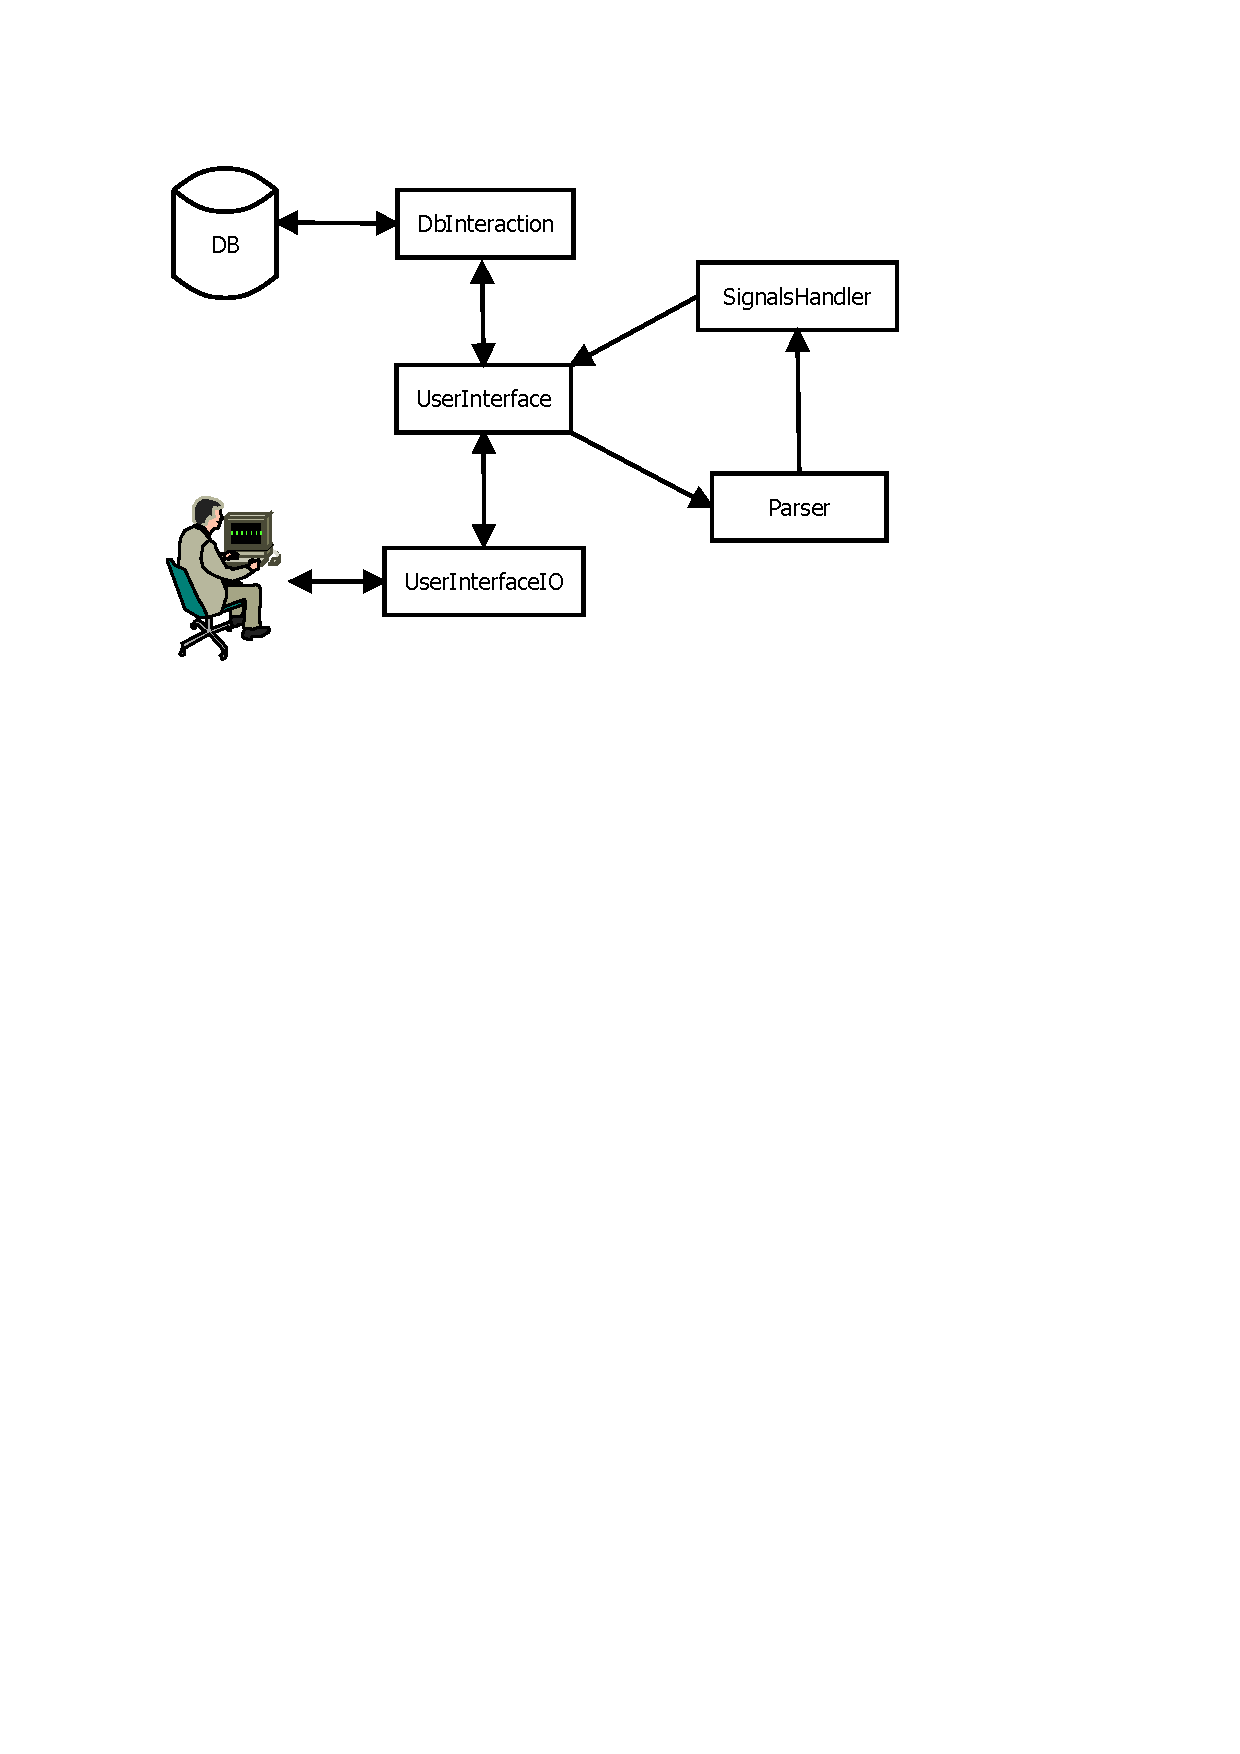
\includegraphics[trim=28mm 182mm 57mm 28mm, clip=true]{img-deska-cli.pdf}
    \caption{Deska CLI Structure}
\end{figure}

Now we can describe all components in more detail.

\section{DbInteraction}

In the CLI part of Deska are used specific structures for manipulating data from the DB. We will describe firstly 
these structures, and then the role of {\tt DbInteraction}.

\subsection{Structures}

First structure is {\tt AttributeDefinition}. This one is very simple. It is containing attribute name ({\tt Db::Identifier}))
and its value ({\tt Db::Value}). {\tt AttributeDefinition} is not fully determined by itself as it 
does not contain any information about object to which this attribute with value belongs. So another structure is {\tt ObjectDefinition}.
This one is very similar to {\tt AttributeDefinition}, because it is also representing some kind of 
key - value structure. It contains kind name ({\tt Db::Identifier})) and object name ({\tt Db::Identifier})). The name 
is fully qualified, so in case of one object embedded using relations to another, this name will contain symbol {\tt ->} 
and both names. For example when we imagine kind "host" and embedded kind "interface". We can have one host -- "hpv2" 
and its "interface" -- "eth0". Now the {\tt ObjectDefinition} for this interface will have kind "interface" and name 
"hpv2->eth0". And now, when we have pair of {\tt AttributeDefinition} and {\tt ObjectDefinition}, we perfectly know, 
what value of which attribute belongs to a specific object. These structures are used for both assigning and obtaining 
the attributes from DB or creating objects. Another structure is a little bit more complicated. It is {\tt ContextStack}
and {\tt ContextStackItem}. {\tt ContextStack} is only a simple {\tt std::vector} of {\tt ContextStackItem} instances.
Under {\tt ContextStack} you can imagine some kind of path in directory structure on your computer where one item is not
a folder, but it is an object. When we use our example of {\tt ObjectDefinition}, the {\tt ContextStack} representing
the "interface eth0" will have two instances of {\tt ContextStackItem}: "host hpv2" and "interface eth0". You can see,
that in opposite to the {\tt ObjectDefinition}, {\tt ContextStackItem} is not fully qualified by itself. You must have
the whole {\tt ContextStack} in order to know which object is it representing. Till now we were talking about
{\tt ContextStack} representing only one object. In this case, {\tt ContextStack} contains only something like
instances of {\tt ObjectDefinition} without fully qualified names. {\tt ContextStackItem} could also represent a filter.
In this case it is a pair of kind name and {\tt Db::Filter}. Using context stack with a filter you can address a set of
objects with a specific characteristic. For example all interfaces of object "host hpv2" that belongs to a specific
network.

Because the work in the CLI is based mostly on the context stack as it is a natural way how to deal with the structure
of data in the DB and DBAPI is based on functions working with single objects or filters, we have the implemented the
class {\tt DbInteraction} to deal with conversion from context stack to format that is suitable for DBAPI.

\subsection{Context stack conversion}

As we described earlier, the context stack can be simple, without filters or more complicated with filters.

Conversion of {\tt ContextStack} to a single {\tt ObjectDefinition} is possible only when the {\tt ContextStack} does
not contain any filters. This type of conversion is very straight forward and could be done without queries to the DB.
We simply concatenate all object names from the stack with {\tt ->} symbol and use kind name from the last kind in the stack.

When we want to convert {\tt ContextStack} with filters, we have to perform queries to the DB. The conversion is made
step by step when going through the stack. In every time of the conversion we have a vector of all objects matching current
level of context stack. When the {\tt ContextStackItem} is representing an object, we only extend all names in the vector
with the {\tt ->} symbol and the object name from the {\tt ContextStackItem} and use kind name from the {\tt ContextStackItem}.
When the {\tt ContextStackItem} is representing a filter, we have to construct a large filter. Firstly we have to construct
a filter matching all objects in the vector. This is done by {\tt Db::OrFilter} containing all object names. Then we use
this filter together with filter from {\tt ContextStackItem} in a {\tt Db::AndFilter}. Now we have filter matching new
level of context stack, that can be used for performing operations through DBAPI.

\subsection{Caching}

Another role of class {\tt DbInteraction} is caching of several types of data to reduce computing time, server load and delays.
This is because of the fact, that CLI uses the information provided by a server in a specific way that does not correspond
with the format obtained from the server.

First caching is made on DB structure. {\tt DbInteraction} stores names of kinds and their attributes in several maps
(we used nested {\tt std::map} for implementation of these structures) for fast access to data needed for operations with
the DB. Information like to which kind each attribute refers, in which kind is some kind embedded and more are stored
here. This is the caching made because of the format of the data.

Another caching is performed on queries checking if some object exists or not, as these queries are quite frequent.
Because all queries to the DB are performed through this class, we can update our cache while performing modification to
the DB like creating objects, deleting objects, renaming objects and so on. This one reduces server load and network traffic.

\section{UserInterface}

Class {\tt UserInterface} is the central class holding the logics of the CLI. This class serves like a glue connecting
all other components together.

It is driven by two types of commands. First type are commands implemented as classes inherited from {\tt Command}.

\begin{minted}{c++}
class Command
{
public:
    Command(UserInterface *userInterface);
    virtual ~Command();
    virtual bool operator()(const std::string &params) = 0;
protected:
    std::vector<std::string> complPatterns;
    std::string cmdName;
    std::string cmdUsage;
};
\end{minted}

As you can see, the base is very simple. In constructor several mandatory variables of the class are set like
completion patterns, command name, and usage description for help generation. These commands are influencing the rest of
the Deska through pointer to {\tt UserInterface}. These command classes are stored in a map with their names as a key.
After that they are picked up using this name. Executing the command is made by calling function {\tt bool operator()} with
string as a parameter. This parameter could be then processed to influence behavior of each command. Return value is here
to tell the other world is the executing of the command succeeded or not. Names and parameters of these commands
are independent on DB structure. Their purpose are things like operations with changesets, dumping, backuping and restoring
the DB and so on. We will describe each command separately in more detail later.

The second type of commands are dependent on DB structure. They are used for manipulating data in the DB like setting attributes,
creating, deleting and renaming objects and so on. Because of the fact, that these actions are performed using calls
like {\tt <attribute-name> <attribute-value>} or {\tt <kind-name> <object-name>}, you can see, that here actually is not any
name for this command. It is fully determined by the action it should perform. A special class was developed for parsing
of these "commands", class {\tt Parser}. It is one of the main components and also one of the most complicated, so we will
describe it later in a separate section. The parser itself does not change the data in the DB. It communicates with the
{\tt UserInterface} through simple class {\tt SignalsHandler}. This class is here because the parser emits signals for
each action. These signals are caught and stored in the {\tt SignalsHandler}. Then comes two way processing of the stack,
where in the first round each action represented by one signal is confirmed and then when all signals are confirmed, they
are applied to the DB. The confirmation and applying is performed via functions implemented in the {\tt UserInterface},
that you can see on the following snippet.

\begin{minted}{c++}
class UserInterface: public boost::noncopyable
{
public:

...

    bool applyCreateObject(const ContextStack &context,
            const Db::Identifier &kind, const Db::Identifier &object, ContextStackItem &newItem);
    bool applyCategoryEntered(const ContextStack &context,
            const Db::Identifier &kind, const Db::Identifier &object, ContextStackItem &newItem);
    bool applySetAttribute(const ContextStack &context, const Db::Identifier &kind,
            const Db::Identifier &attribute, const Db::Value &value);
    bool applySetAttributeInsert(const ContextStack &context, const Db::Identifier &kind,
            const Db::Identifier &attribute, const Db::Identifier &value);
    bool applySetAttributeRemove(const ContextStack &context, const Db::Identifier &kind,
            const Db::Identifier &attribute, const Db::Identifier &value);
    bool applyRemoveAttribute(const ContextStack &context, const Db::Identifier &kind,
            const Db::Identifier &attribute);
    bool applyObjectsFilter(const ContextStack &context, const Db::Identifier &kind,
            const boost::optional<Db::Filter> &filter);
    bool applyFunctionShow(const ContextStack &context);
    bool applyFunctionDelete(const ContextStack &context);
    bool applyFunctionRename(const ContextStack &context, const Db::Identifier &newName);

    bool confirmCreateObject(const ContextStack &context,
            const Db::Identifier &kind, const Db::Identifier &object);
    bool confirmCategoryEntered(const ContextStack &context,
            const Db::Identifier &kind, const Db::Identifier &object, bool &autoCreate);
    bool confirmSetAttribute(const ContextStack &context, const Db::Identifier &kind,
            const Db::Identifier &attribute, const Db::Value &value);
    bool confirmSetAttributeInsert(const ContextStack &context, const Db::Identifier &kind,
            const Db::Identifier &attribute, const Db::Identifier &value);
    bool confirmSetAttributeRemove(const ContextStack &context, const Db::Identifier &kind,
            const Db::Identifier &attribute, const Db::Identifier &value);
    bool confirmRemoveAttribute(const ContextStack &context, const Db::Identifier &kind,
            const Db::Identifier &attribute);
    bool confirmObjectsFilter(const ContextStack &context, const Db::Identifier &kind,
            const boost::optional<Db::Filter> &filter);
    bool confirmFunctionShow(const ContextStack &context);
    bool confirmFunctionDelete(const ContextStack &context);
    bool confirmFunctionRename(const ContextStack &context, const Db::Identifier &newName);

...

};
\end{minted}

Now we will describe how the more complicated commands from the first group work.

\subsection{Rebase}

\todo{Tomas: Rewrite in more detail}

Class {\tt Rebase} is quite complicated one. It's purpose is to reconnect current changeset from its parent to a new
one. This is done firstly by creating a new changeset, which will be connected to a newest revision and then by performing
the same changes as we performed in old changeset in this changeset. Then we can abort the old changeset. Well we can not
perform exactly the same changes in our new changeset, because the DB could change that it could not be possible. For
example when we set attribute of some object which was deleted in a newer revision. To solve this problem we are performing
some kind of merge here. We obtain two sets of {\tt Db::ObjectModificationResult}. Firs is diff between our old changeset
and its parent. This gives us list of our changes. Next set is diff between parent of our old changeset and parent of a
new changeset. This represents changeset made while we were working in our old changeset. These sets has to be somehow
merged and shown to a user in order to see, haw the final result of merge will look like and also in order to influence
the result of this merge. The merge is performed by several comparators and the result has to be in the following order:
\begin{enumerate}
    \item {\tt Db::DeleteObjectModification}
    \item {\tt Db::RenameObjectModification}
    \item {\tt Db::CreateObjectModification}
    \item {\tt Db::SetAttributeModification}
\end{enumerate}
This order was chosen because of constraints in the DB. For example when we are creating some object, the object with
the same name must not exist and so on. So deleting does not break any constraint any time. Rename is before create
because you can create then the object of the same name as an old one, but you will never need to perform create before
rename to unblock rename. Setting attributes must be last as it requires an existing object. After this sorting and
merging the result is shown to the user using an interactive editor implemented in {\tt UserInterfaceIO}. Here the user
can delete or modify the modifications. When the editing part is finished, the corrected list is processed and
all modifications are performed.

\subsection{Log}

Function {\tt bool Log::operator()} when executed without parameters only obtains list of all revisions in the DB and
prints this list using {\tt UserInterfaceIO} to the screen. The more interesting part of this class is parameters parser.
It is based on {\tt boost::spirit} as well as the {\tt Parser}. Parsing of parameters is done by class {\tt LogFilterParser}.
An output of this class is a {\tt Db::Filter}, that will be used directly for obtaining the list of revisions and similarly
printed using {\tt UserInterfaceIO} to the screen. Now we will describe the {\tt LogFilterParser}.

This class is inherited from {\tt boost::spirit::qi::grammar}. The grammar is based on three symbols tables with lazy lookup
function. This method could be found under name "Nabialek trick". We have to use this method as the grammar is build at
the runtime. This is because of the fact, that we have to parse kind names, that are not known at compile time, but are obtained
from the DB. In the first symbols table there are names of metadata (author, timestamp, ...) and is filled at compile time
directly in the constructor. The second one is empty and will be filled using function {\tt void addKind(const Db::Identifier \&kindName)}.
The third table contains operators. This parser is connected to three error handlers. {\tt LogAttributeErrorHandler}
for reporting an error while parsing an metadata name or a kind name, {\tt LogIdentifierErrorHandler} for reporting errors
while parsing of an object name and {\tt LogValueErrorHandler} for reporting an error while parsing a value of some
metadata. The {\tt boost::spirit} error handlers ale classes with function {\tt operator()}, that will be invoked every time
when the matching of the input to a specific rule fails. Each rule could have associated a number of error handlers. The
problem of this way how error handlers work is, that when some rule fails, error handlers of other rules containing this one
will be cascadely invoked. So we have to store all there errors in a stack and when some error occurs process this stack
and inform user with a proper message. The whole grammar is build as a recursive expression parsing the input directly in the
recursive filers represented by {\tt Db::Filter}. You can see the logics on the following snippet:

\begin{minted}{c++}
start %= ((qi::lit("(") >> andFilter >> qi::lit(")"))
        | (qi::lit("(") >> orFilter >> qi::lit(")"))
        | (qi::lit("(") >> expr >> qi::lit(")")));

andFilter = (start % qi::lit("&"))[_val = phoenix::construct<Db::AndFilter>(_1)];
orFilter = (start % qi::lit("|"))[_val = phoenix::construct<Db::OrFilter>(_1)];

expr %= kindExpr | metadataExpr;

kindExpr %= (eps(!_a) > kindDispatch >> -eoi[_a = true]);
metadataExpr %= (eps(!_a) > metadataDispatch >> -eoi[_a = true]);

// Kind name recognized -> try to parse object name
kindDispatch = (raw[kinds[_a = _1]][rangeToString(_1, phoenix::ref(currentKindName))]
    > operators[_b = _1] > lazy(_a)[_val = phoenix::construct<Db::AttributeExpression>(
        _b, phoenix::ref(currentKindName), "name", phoenix::construct<Db::Value>(_1))]);
// Metadata name recognized -> try to parse metadata value
metadataDispatch = (raw[metadatas[_a = _1]][rangeToString(_1, phoenix::ref(currentMetadataName))]
    > operators[_b = _1] > lazy(_a)[_val = phoenix::construct<Db::MetadataExpression>(
        _b, phoenix::ref(currentMetadataName), _1)]);
        
phoenix::function<LogAttributeErrorHandler<Iterator> > attributeErrorHandler
    = LogAttributeErrorHandler<Iterator>();
phoenix::function<LogValueErrorHandler<Iterator> > valueErrorHandler
    = LogValueErrorHandler<Iterator>();
phoenix::function<LogIdentifierErrorHandler<Iterator> > identifierErrorHandler
    = LogIdentifierErrorHandler<Iterator>();
on_error<fail>(kindExpr, attributeErrorHandler(_1, _2, _3, _4,
    phoenix::ref(kinds), phoenix::ref(metadatas), m_parent));
on_error<fail>(metadataExpr, attributeErrorHandler(_1, _2, _3, _4,
    phoenix::ref(kinds), phoenix::ref(metadatas), m_parent));
on_error<fail>(kindDispatch, identifierErrorHandler(_1, _2, _3, _4,
    phoenix::ref(currentKindName), m_parent));
on_error<fail>(metadataDispatch, valueErrorHandler(_1, _2, _3, _4,
    phoenix::ref(currentMetadataName), m_parent));
\end{minted} 

When parsing some input using Nabialek trick, the rule, that is using the symbols table will not be entered when the keyword
is not found in the table. The {\tt eps} is there to ensure, that the {\tt kindExpr} and {\tt metadataExpr} rules will be
entered every time and so the error handler for bad keywords could be bound to it. The {\tt eoi} rule is there to avoid
the grammar require more input on the end of the line, which is side effect of eps usage in this way.

\subsection{Diff}

This function obtains list of {\tt Db::ObjectModificationResult} between two revisions or between changeset and its parent.
This depends on the parameters given. The output depends on the destination. If it is a diff to file the modifications
are sorted in the way like in {\tt Rebase}. This is because of the fact, that this output of the diff could be used for
example for backing the work in the changeset up. So we have to for example create the object before we are referencing it
in another object. This form of output is unfortunately not very user friendly. When the destination is a screen, the
modifications are sorted in the way, that modifications of one objects are grouped. This allows us to better illustrate
the obtained modifications.

\subsection{Dump}

Dump is performing some visual picture of the whole DB. The output is the same when dumping to the file or to the screen.
It is not intended to be used for backing anything up as it does not take any constraints in account.
The principle is very simple. We have a list of all kinds that could not be embedded in any other. This gives us a list
of "top-level" kinds. Now we can obtain instances of these kinds and for each instance we obtain list of embedded objects.
This is performed recursively. As the embedded objects can not live without their parents, we can print all objects in this way.

\subsection{Batch}

Class {\tt Batch} reads and performs commands readable by the {\tt Parser} from a file. It could be used for reading of
an output from a diff.

\subsection{Backup}

Command {\tt backup} is here to backup all persistent revisions from the DB including data. This is performed by obtaining
differences between each two revisions and saving these differences in a file. The order of the modifications is the same
as in case of diff to a file.

The format of the backup is following:

\begin{minted}{text}
<list of modifications between r1 and r2, one per line>
...
@commit to r2
<author>
<commit message>
<commit timestamp>
#commit end
<list of modifications between r2 and r3, one per line>
...
@commit to r3
<author>
<commit message>
<commit timestamp>
#commit end
...
\end{minted}

\subsection{Restore}

Restore reads backup created by {\tt Backup}. Restore is performed using function {\tt RevisionId restoringCommit(const
std::string \&commitMessage, const std::string \&author, const boost::posix\_time::ptime \&timestamp)}. The DB has to be empty
in order to perform restore. This is checked before any actions are made.

\subsection{Execute}

Command {\tt execute} was implemented mainly for testing purposes. It reads commands from a file and performs actions. It
can read the same commands, that can be written to the CLI. The only difference is, that all command run in non-interactive
mode. This means, that user will not be asked for any confirmations as this would be impossible when reading commands from
a file.

\subsection{Help}

Help collects all help entries from the {\tt Parser} and from all registered CLI commands and sends all these entries to the
{\tt UserInterfaceIO} that will print these entries in a nice form to the user.

\subsection{Other commands}

There is a bunch of other commands, that are not very interesting. You can see a reference inline comments for more info.
Their names are {\tt Start}, {\tt Resume}, {\tt Commit}, {\tt Detach}, {\tt Abort}, {\tt Status}, {\tt NonInteractive},
{\tt Configdiff}, {\tt Exit}, {\tt Context}.

\section{Parser}

The {\tt Parser} parses lines in the CLI, that does not begin with name of some command implemented through class {\tt Command}.
The actions, you can perform though this parser do not depend only on the command written to the CLI, but also on the
context in which the parser currently is. It is based on many sub parsers stored in maps and calculated depending on the current context.

The whole parser operates in one loop. At the beginning, before the loop, it tries to parse function words using
{\tt functionWordsParser} to switch the parsing mode. It means whether the whole kinds including attributes definitions
or only kind definitions will be parsed etc. After parsing the function words, parser will step into the main loop.

Here the grammars are invoked until the whole line is parsed or until some parse error occurs. We have to parse
the line in such loops because we are allowing so called inline operations. That means we can step into context of
a object and set attributes of this object using only one line. Setting an attribute value requires the parser to
be in context of the object, which attribute are we going to set. So as you can see, context before parsing and
during parsing can differ. The loops ensures, that after each parsed kind definition, the parsing is terminated so
parser could change the parsing context and continue parsing by taking another grammar for the new context.
The main loop terminates when the grammars in this loop fail or if the whole line was parsed.

After this main loop, the parser could take some more actions depending on the parse mode. For example parsing of
a new name when renaming some object. After these actions the actual parsing finishes.

Now we check whether the parsing succeeded or not. Each sub parser is connected to several error handlers that
generate parse errors (instances of class {\tt ParseError}) and store them in a stack. If the parsing fails, we can find
the reason in this stack. So when this situation happens, {\tt reportParseError()} function is called to process
the errors stack and report the error.

The whole parser communicates with the outer world through emitting the signals of the parent parser.

\begin{itemize}
    \item {\tt PredefinedRules} -- parser for attribute values
    \item {\tt AttributeRemovalsParser} -- parsing commands removing an attribute value
    \item {\tt AttributesSettingParser} -- parsing commands setting a value of an attribute 
    \item {\tt IdentifiersSetsParser} -- parsing operations with identifier sets - additions and removals of single items
    \item {\tt AttributesParser} -- parser connecting {\tt AttributesSettingParser}, {\tt AttributeRemovalsParser} and
                                    {\tt IdentifiersSetsParser} together 
    \item {\tt FunctionWordsParser} -- parsing function words {\tt create}, {\tt delete}, {\tt rename} and {\tt show}
    \item {\tt KindsOnlyParser} -- parsing object definitions
    \item {\tt KindsConstructParser} -- parsing object creations with automatic name construction
    \item {\tt FilterExpressionsParser} -- parser creating one {\tt Db::AttributeExpression}, it means it parses comparisons between
                                           attribute names and their values
    \item {\tt FiltersParser} -- parser for regular filters for one specific kind employing {\tt FilterExpressionsParser}, this one parses
                                 their conjuction and disjunction with braces 
    \item {\tt KindsFiltersParser} -- parser connecting {\tt FiltersParser} and special filter parsers like {\tt all} 
    \item {\tt KindsParser} -- parser combining {\tt KindsOnlyParser}, {\tt KindsConstructParser} and {\tt FiltersParser}
    \item {\tt WholeKindParser} -- parser combining {\tt KindsParser} and {\tt AttributesParser}  
    \item {\tt TopLevelParser} -- parser combining {\tt KindsOnlyParser} and \item {\tt KindsFiltersParser}
\end{itemize}

Figure \ref{img:deska-cli-parser} shows the structure of the parser. Arrows are showing, where the parser is used. Only the blue
ones are used for parsing of an actual input. Others are only parts (sub-parsers) of other bigger units.

\begin{figure}[h]
    \centering
    \label{img:deska-cli-parser}
    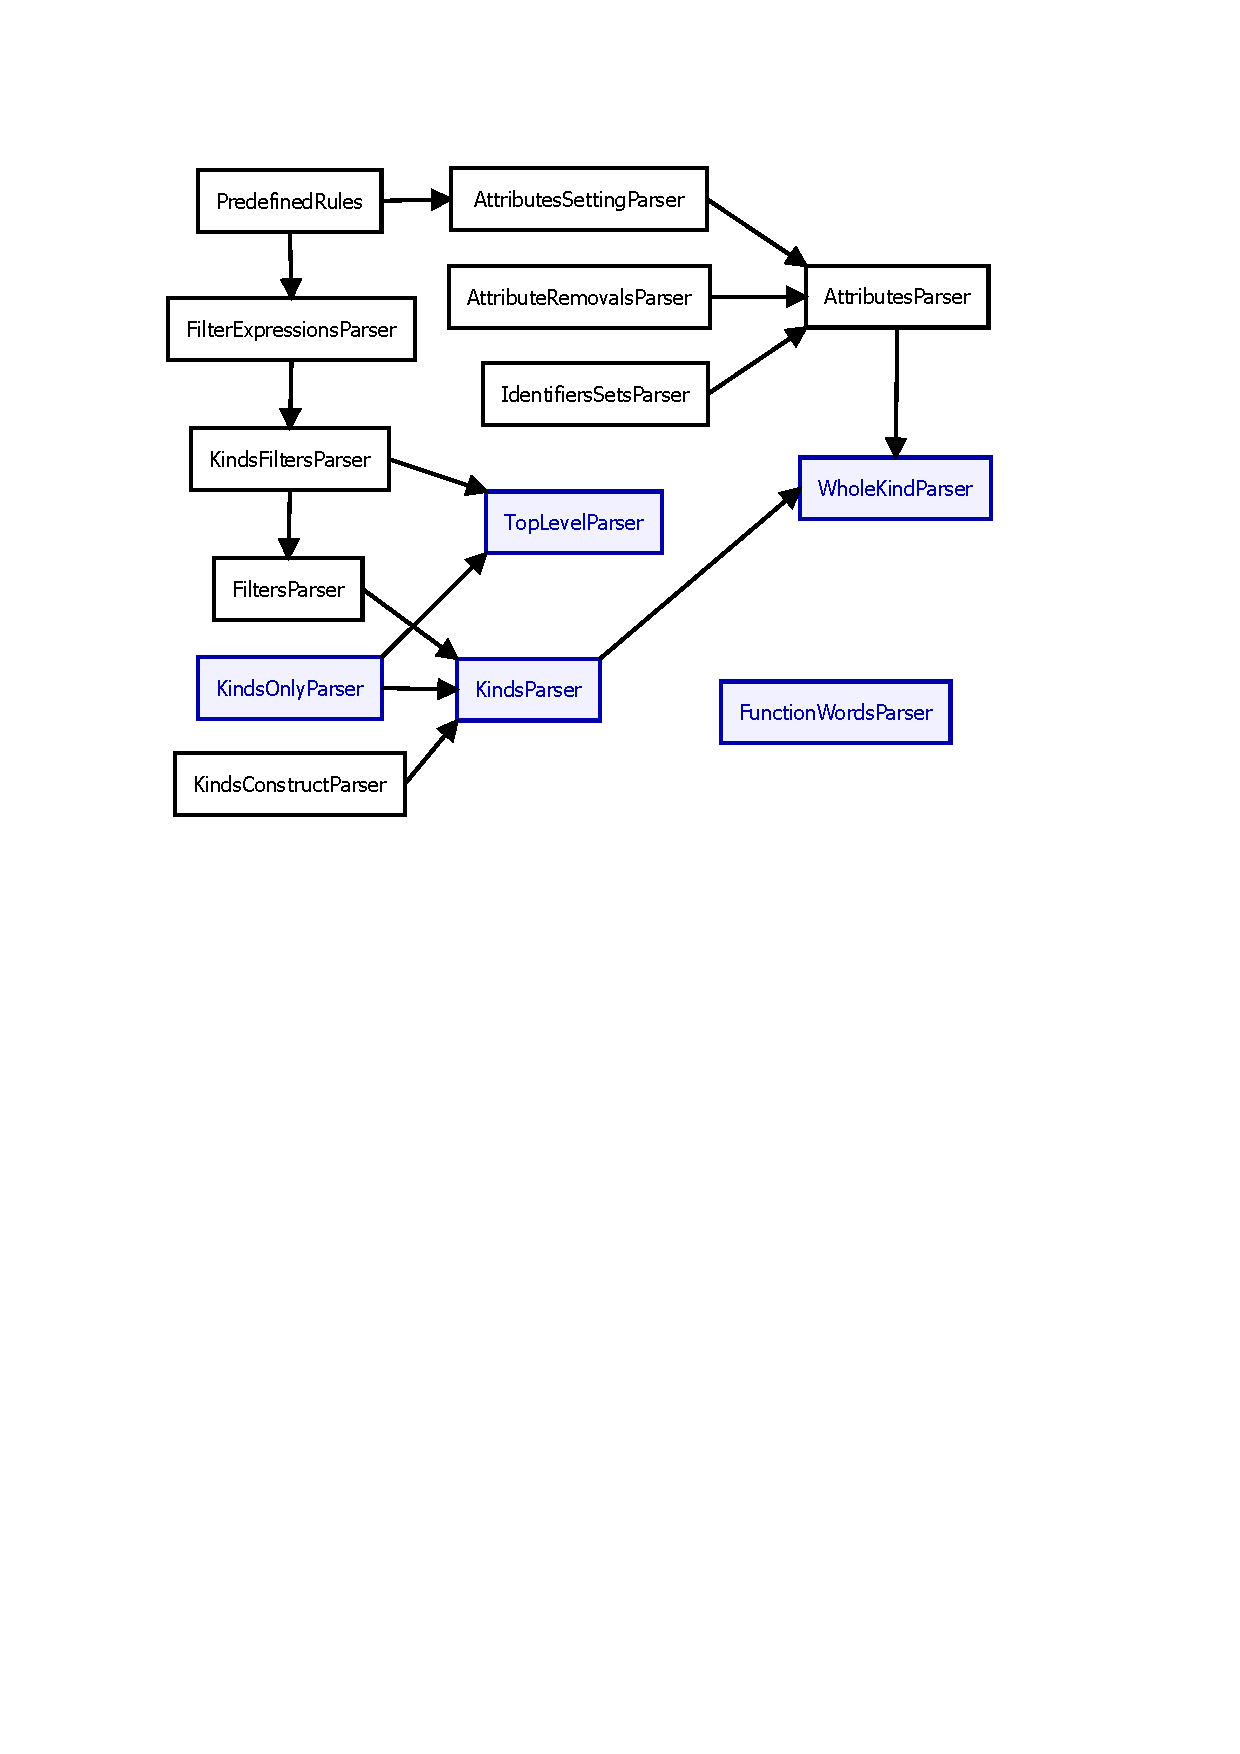
\includegraphics[trim=28mm 157mm 41mm 28mm, clip=true]{img-deska-cli-parser.pdf}
    \caption{Deska CLI Parser}
\end{figure}

Now we will describe the single sub-grammars and error reporting in more detail.

\subsection{PredefinedRules}

Class {\tt PredefinedRules} contains definitions of rules parsing values of all defined types. These rules are stored
in the map indexed by a {\tt Db::Type}. It also contains rules for all metadata types used in revisions and changesets
like parser of timestamps, revisions IDs, temporary changeset IDs and so on. You can see reference manual for more details.
Each rule has assigned its name used in error reporting.

If some would like to extend the Deska with more data types, he has to implement also rule for parsing of this datatype
and store it under appropriate {\tt Db::Type}. Nothing more is needed.

\subsection{AttributeParser}

As we wrote, this parser consists of {\tt AttributesSettingParser}, {\tt AttributeRemovalsParser} and {\tt IdentifiersSetsParser}.
This is made by operator "or".

{\tt AttributesSettingParser} parses only one pair from set of <attribute\_name> <attribute\_value> definitions, {\tt AttributeRemovalsParser}
parses a pair {\tt no <attribute\_name>} and {\tt IdentifiersSetsParser} parses commands like {\tt add <set\_name> <identifier>} or
{\tt remove <set\_name> <identifier>}. Parsing only one pair does not mean that this parser accepts only
one attribute. It means, that parse accepts any attribute of a specific kind, but not a list of them.
For parsing set of these pairs, use some {\tt boost::spirit} operator like Kleene star.

All these grammars are based on a symbols tables with lazy lookup function. This method could be found
under name "Nabialek trick". This is the same trick as we used in {\tt LogFilterParser}. Each parsed comand is sent to the
main parser (parent) using semantic actions {\tt parsedAttribute()}, {\tt parsedAdd()} or {\tt parsedRemove()}.

These parsers are connected to error handlers {\tt AttributeRemovalErrorHandler}/{\tt AttributeErrorHandler} for reporting an error
while parsing an attribute name, {\tt IdentifiersSetsErrorHandler} for reporting an error while parsing a set name and
{\tt ValueErrorHandler} for reporting an error while parsing a value of an attribute.

There is one {\tt AttributeParser} with sub-parsers for each kind.

\subsection{FunctionWordsParser}

Function words parser is a stand-alone parser outside of the main parsing loop. As we wrote, this one parses function words
{\tt create}, {\tt delete}, {\tt rename} and {\tt show}. Each parsed keyword is reported by appropriate function call that changes parsing mode.
For example when keyword {\tt delete} was recognized, the rest of the input will be parsed only by {\tt KindsParser}. It means
no operations with attributes will be allowed for th rest of the line.

\subsection{KindsOnlyParser and KindsConstructParser}

These two parsers uses the same trick as parsers for attributes, the "Nabialek trick". {\tt KindsConstructParser} parses
a pair of {\tt new <kind\_name>}. This is used for creating objects where the name of these objects is not important and we
want the DB to generate it. This action is reported by semantic action {\tt parsedObjectCreation()}. This parser is connected
to one error handler, {\tt KindConstructErrorHandler} for reporting an error while parsing a kind name.

{\tt KindsOnlyParser} differs from the {\tt KindsConstructParser} with parsed command and semantic action. This one parses
pair <kind\_name> <object\_name> and the semantic action is {\tt parsedKind()}. This parser is connected to two error handlers.
{\tt KindErrorHandler} for reporting an error while parsing a kind name and {\tt ObjectNameErrorHandler} for reporting an
error while parsing an object name.

There is also one {\tt KindsOnlyParser} and {\tt KindsConstructParser} for each kind. 

\subsection{FiltersParser}

{\tt FiltersParser} works, as all other grammars, on basis of "Nabialek trick". Here the trick is a little bit tuned up.
Normally this trick works on symbols table with rules. It is not possible to do it on grammars as symbols tables are not
able to work with them. {\tt Spirit} allows to assign a {\tt qi::grammar} to a {\tt qi::rule}. This creates a reference
to the grammar stored in this rule. Now we can store this rule in a symols table and use "Nabialek trick" with grammars.

Each kind has its own {\tt FiltersParser}. This parser has one {\tt FilterExpressionsParser} for parsing of filters
on own attributes and symbols table is filled with instances of {\tt FilterExpressionsParser} for filters on attributes
of somehow connected kinds (by relations). The symbols table is indexed by kind name and each parser is then accessed
using kind name and dot. For example {\tt interface.ipv4 == 192.168.1.1}. The structure of the {\tt FiltersParser} is quite
well ilustrated by the following code snippet.

\begin{minted}{c++}
start %= ((qi::lit("(") >> andFilter >> qi::lit(")"))
        | (qi::lit("(") >> orFilter  >> qi::lit(")"))
        | (qi::lit("(") >> attrExpr  >> qi::lit(")")));

andFilter = (start % qi::lit("&"))[_val = phoenix::construct<Db::AndFilter>(_1)];
orFilter = (start % qi::lit("|"))[_val = phoenix::construct<Db::OrFilter>(_1)];

attrExpr %= (*ownAttrsExpressionsParser) | nestedAttrExpr;

nestedAttrExpr %= (eps(!_a) > dispatch >> -eoi[_a = true]);

// Nested kind name recognized -> try to parse expression for the kind. The raw function is
// here to get the name of the kind for which the expression is being parsed.
dispatch = (raw[nestedAttributes[_a = _1]][rangeToString(_1, phoenix::ref(nestedKindName))] >
           qi::lit(".") > lazy(_a))[_val = _2];

phoenix::function<KindFiltersErrorHandler<Iterator> > kindFiltersErrorHandler
    = KindFiltersErrorHandler<Iterator>();
on_error<fail>(nestedAttrExpr, kindFiltersErrorHandler(_1, _2, _3, _4,
    phoenix::ref(nestedAttributes), phoenix::ref(m_name), m_parent));
\end{minted}

{\tt KindFiltersErrorHandler} is used for reporting an error while parsing a name of a related kind.

Now we can describe the {\tt FilterExpressionsParser}. This parser is based on two symbols tables. One for sets and another
for normal attributes as the operators, that can be used for them differ. The internal structure of this parser is well
readable, so we can attach a code snippet.

\begin{minted}{c++}
operators.add("=", Db::FILTER_COLUMN_EQ);
operators.add("==", Db::FILTER_COLUMN_EQ);
operators.add("!=", Db::FILTER_COLUMN_NE);
operators.add("<>", Db::FILTER_COLUMN_NE);
operators.add(">", Db::FILTER_COLUMN_GT);
operators.add(">=", Db::FILTER_COLUMN_GE);
operators.add("<", Db::FILTER_COLUMN_LT);
operators.add("<=", Db::FILTER_COLUMN_LE);

setsOperators.add("contains", Db::FILTER_COLUMN_CONTAINS);
setsOperators.add("not_contains", Db::FILTER_COLUMN_NOT_CONTAINS);

start %= (eps(!_a) > dispatch >> -eoi[_a = true]);

dispatch %= dispatchAll | dispatchSets;

// Attribute name recognized -> try to parse filter value. The raw function is here to
// get the name of the attribute being parsed.
dispatchAll = (raw[attributes[_a = _1]][rangeToString(_1, phoenix::ref(currentAttributeName))] >>
    operators[_b = _1] > lazy(_a)[_val = phoenix::bind(
        &FilterExpressionsParser<Iterator>::constructFilter, this, _b,
            phoenix::ref(currentAttributeName), phoenix::construct<Db::Value>(_1))]);
dispatchSets = (raw[sets[_a = _1]][rangeToString(_1, phoenix::ref(currentAttributeName))] >>
    setsOperators[_b = _1] > lazy(_a)[_val = phoenix::bind(
        &FilterExpressionsParser<Iterator>::constructFilter, this, _b,
            phoenix::ref(currentAttributeName), phoenix::construct<Db::Value>(_1))]);

phoenix::function<AttributeFilterErrorHandler<Iterator> > attributeFilterErrorHandler
    = AttributeFilterErrorHandler<Iterator>();
phoenix::function<ValueErrorHandler<Iterator> > valueErrorHandler = ValueErrorHandler<Iterator>();
on_error<fail>(start, attributeFilterErrorHandler(_1, _2, _3, _4,
    phoenix::ref(attributes), phoenix::ref(sets), phoenix::ref(m_name), m_parent));
on_error<fail>(dispatch, valueErrorHandler(_1, _2, _3, _4,
    phoenix::ref(currentAttributeName), m_parent));
\end{minted}

You can see, that error handler are there the same as in {\tt AttributesSettingParser} and has also the same function here.
Another point to mention here is, that the return value of the rule {\tt start} is the final {\tt Db::AttributeExpression},
that is then processed by {\tt FiltersParser} and more complicated filters are constructed here by conjunction or disjunction
of these {\tt Db::AttributeExpression}s.

\subsection{WholeKindParser and TopLevelParser}

These two parsers only combine another sub-parsers into one. {\tt TopLevelParser} combines {\tt KindsOnlyParser} and
{\tt KindsFiltersParser}. Top-level parser is used every time the {\tt ContextStack} is empty. This parser contains subparsers
of each kind, because you can write a filter for any kind from the top level as well as jump in the context of any kind.

{\tt WholeKindParser} is used for parsing of kinds, when the context stack is not empty. So it combines {\tt AttributesParser}
and also {\tt KindsParser}. Besides these grammars is also keyword {\tt end} parsed here for leaving one level of context.

\subsection{ErrorReporting}

Error reporting is based on collecting all errors from all rules, that have some error handler assigned and then by
processing this stack of errors. Here you can see the mapping of the error types ({\tt enum ParseErrorType}) to
error handlers.

\begin{itemize}
    \item {\tt KindConstructErrorHandler} - {\tt PARSE\_ERROR\_TYPE\_KINDS\_CONSTRUCT}
    \item {\tt KindErrorHandler} - {\tt PARSE\_ERROR\_TYPE\_KIND}
    \item {\tt KindFiltersErrorHandler} - {\tt PARSE\_ERROR\_TYPE\_KIND\_FILTER}
    \item {\tt KindSpecialFiltersErrorHandler} - {\tt PARSE\_ERROR\_TYPE\_KIND\_SPECIAL\_FILTER}
    \item {\tt AttributeErrorHandler} - {\tt PARSE\_ERROR\_TYPE\_ATTRIBUTE}
    \item {\tt AttributeFilterErrorHandler} - {\tt PARSE\_ERROR\_TYPE\_ATTRIBUTE}
    \item {\tt IdentifiersSetsErrorHandler} - {\tt PARSE\_ERROR\_TYPE\_IDENTIFIERS\_SET}
    \item {\tt AttributeRemovalErrorHandler} - {\tt PARSE\_ERROR\_TYPE\_ATTRIBUTE\_REMOVAL}
    \item {\tt ValueErrorHandler} - {\tt PARSE\_ERROR\_TYPE\_VALUE\_TYPE}
    \item {\tt ObjectNameErrorHandler} - {\tt PARSE\_ERROR\_TYPE\_OBJECT\_NAME}
\end{itemize}

Now the errors are reported due to a priority of the error types. As we described while writing about class {\tt Log},
the error handlers are invoked recursively. For example when we are writing an attribute definition and we do some error
in the value, the {\tt ValueErrorHandler} is invoked, but also due to cascading {\tt AttributeErrorHandler} is invoked as well.
That is why we have to process this context stack and not print the error directly from the handler.
The priority of the error types is following:

\begin{enumerate}
    \item {\tt PARSE\_ERROR\_TYPE\_VALUE\_TYPE}
    \item {\tt PARSE\_ERROR\_TYPE\_OBJECT\_DEFINITION\_NOT\_FOUND} - this error is not generated by error handlers, but is
                                                               generated by the main parser when it requires an object definition
                                                               for example for action "delete" or "rename"
    \item {\tt PARSE\_ERROR\_TYPE\_IDENTIFIER\_NOT\_FOUND} - this error is again not generated by any error handler, but by the main
                                                        parser when it expects identifier for action "rename"
    \item {\tt PARSE\_ERROR\_TYPE\_OBJECT\_NOT\_FOUND} - this error is not generated by error handlers, but is
                                                    generated by the main parser when it requires an existing object
    \item {\tt PARSE\_ERROR\_TYPE\_KIND\_NESTING} - this error is generated by main parser when it recognises error while trying
                                                to parse nested kind name when entering context of an object
    \item {\tt PARSE\_ERROR\_TYPE\_KINDS\_CONSTRUCT}
    \item {\tt PARSE\_ERROR\_TYPE\_IDENTIFIERS\_SET}
    \item {\tt PARSE\_ERROR\_TYPE\_ATTRIBUTE\_REMOVAL}
    \item {\tt PARSE\_ERROR\_TYPE\_ATTRIBUTE} - this one could be combined with {\tt PARSE\_ERROR\_TYPE\_KIND} as we are not able
                                             to distinguish between errors in attribute name or nested kind name when
                                             there could be both of them
    \item {\tt PARSE\_ERROR\_TYPE\_OBJECT\_NAME}
    \item {\tt PARSE\_ERROR\_TYPE\_KIND\_SPECIAL\_FILTER}
    \item {\tt PARSE\_ERROR\_TYPE\_KIND}
    \item {\tt PARSE\_ERROR\_TYPE\_KIND\_FILTER}
\end{enumerate}

Final error message with list of possible tokens at the error point is then propagated to the {\tt UserInterface} for reporting.

\section{Tab-completion}

The CLI has tab-completion feature. The tab completion itself is done by the {\tt UserInterfaceIO}. But other components
have to assist while collecting all possibilities. When a user wants to get a list of tab-completions, they are collected
from two places. First is list of static tab-completion patterns from each command (inherited from {\tt Command} registered
in the CLI. Second is list of completions from the parser. This one is more complicated.

The parser has a special mode for obtaining a list of tab completions. It is called "dry run". While parsing some line using
this dry run. No actions are propagated from the parser and after the parsing, the parser remains unchanged including its
context stack. When the parsing succeeds, we are suggesting all keywords depending on the current context stack and line.
Like {\tt show}, {\tt add}, {\tt no}, etc. When the parsing fails, we can process a list of possible tokens from each generated error
and then use these tokens as possible completion patterns. Moreover when the error occurs while parsing an attribute
value, we investigate this attribute if it refers to some kind and then suggest instances of this kind as possible completions.
One more thing to note here is, that also position of the error has to be taken in account as the error could occur somewhere
else, than where we have out cursor. In this case we do no suggest any completions as the error is somewhere before the
cursor.

\section{UserInterfaceIO}

{\tt UserInterfaceIO} is the class handling all IO operations from and to the user. It contains set of function for asking
user for several confirmations, set of function for printing various information. Most of these functions does not
contain any advanced logics. This is centred in {\tt UserInterface}.

{\tt UserInterfaceIO} takes care of tab-completion. For these purposes it uses class {\tt CliCompleter} that obtains completion
patterns from the parser and from the CLI commands. For the logics of tab-completion takes care class {\tt ReadlineWrapper::Readline}.
This is only a C++ wrapper for a well known library {\em readline}. It does splitting of the line to tokens and then comparing
these tokens with given tab-completions patterns to find out matching completions.


\end{document}
